\documentclass[10pt]{beamer}

%STANDARD PREAMBLE
%https://tex.stackexchange.com/questions/68821/is-it-possible-to-create-a-latex-preamble-header
\usepackage{/Users/miw267/Repos/latex_preamble/beamer_preamble}
%\usepackage{/Users/miw267/Repos/csci246_spring2025/slides/preambles/beamer_preamble_for_CSCI246}


%%%
% SPECIFIC TO THIS DOCUMENT 
%%%
\usepackage{animate}

\renewcommand{\ELBO}{\texttt{ELBO}}
\renewcommand{\Q}{\mathcal{Q}}


%%%%
% DOCUMENT 
%%%
\title{04/28/2026: Probabilistic Weather Forecasting}
\author{Reference: \textit{Probabilistic Weather Forecasting with Machine Learning}}
\date{CSCI 546: Diffusion Models}

\begin{document}
\maketitle

%\begin{frame}{Table of contents}
%  \setbeamertemplate{section in toc}[sections numbered]
%  \tableofcontents[hideallsubsections]
%\end{frame}

\begin{frame}{Table of contents}
  \setbeamertemplate{section in toc}[sections numbered]
  \setbeamertemplate{subsection in toc}[subsections numbered]
  \tableofcontents
\end{frame}





\section{Reading Surveys}




\begin{frame}{Reading Survey \#10: Feedback}

\textbf{Original Question:} How do the authors propose imputing missing values in time series data?

\vfill 

\textbf{Feedback:} The core technique is \alert{conditional} diffusion.  We model the probability distribution of missing data conditioned on observed data.  \pause See blackboard for key idea.  \pause  For reference, compare equations (2) and (5) in the paper. 
\end{frame}

\begin{frame}

\begin{figure} 
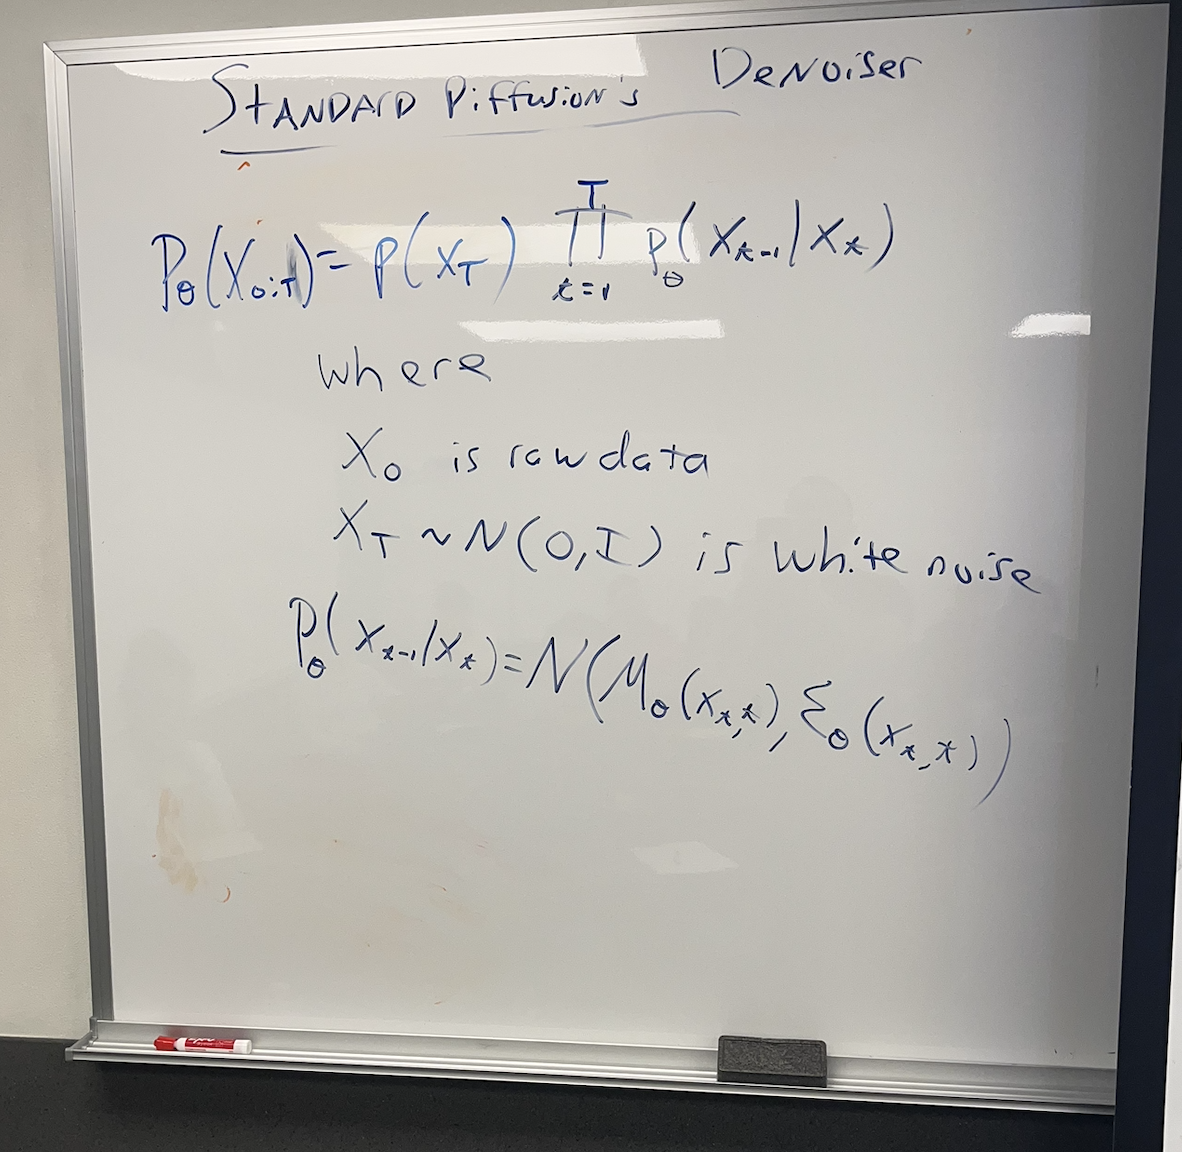
\includegraphics[width=.8\textwidth]{images/conditional_diffusion_1} 
\end{figure}
\end{frame}


\begin{frame}

\begin{figure} 
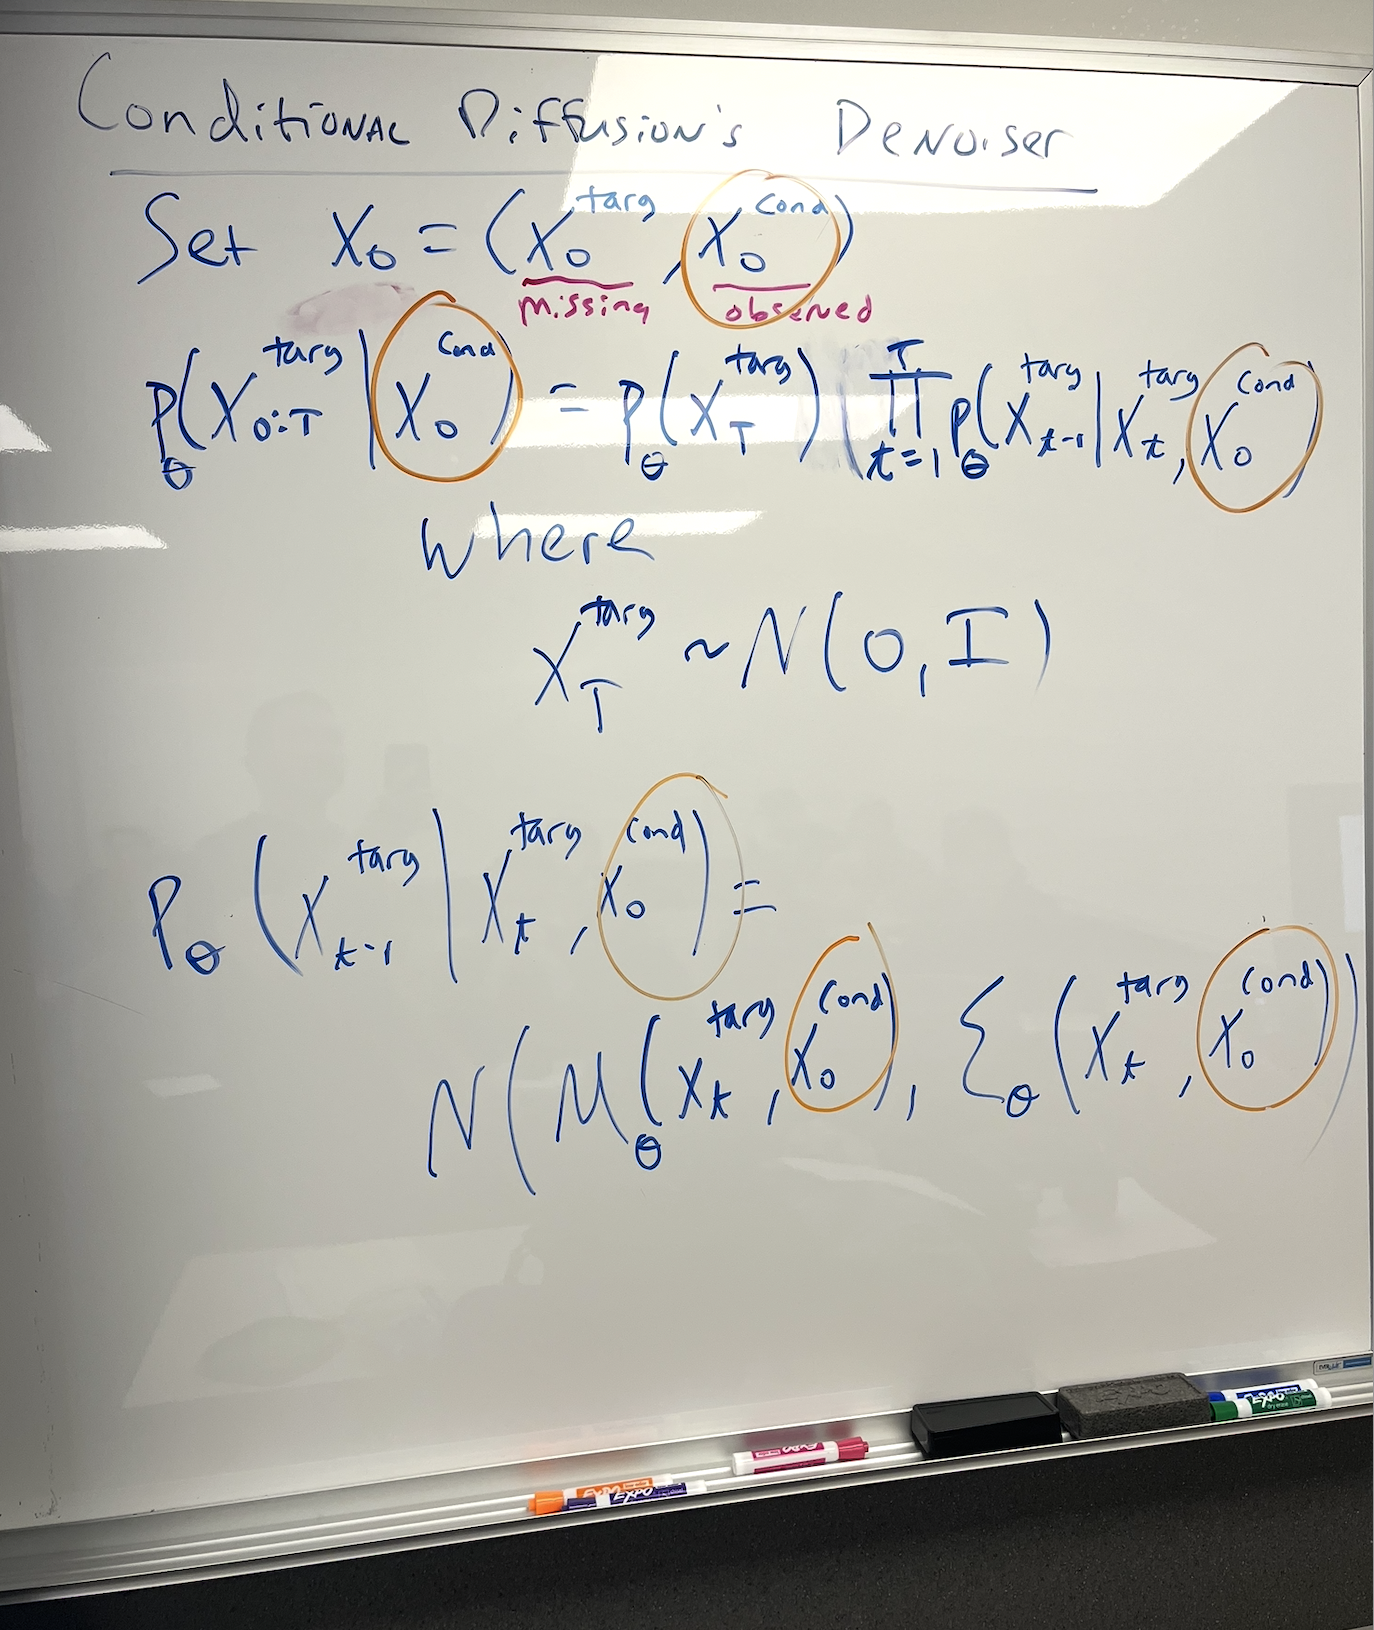
\includegraphics[width=.8\textwidth]{images/conditional_diffusion_2} 
\end{figure}
\end{frame}

\begin{frame}{Reading Survey: Reminder}

\begin{myredbox}[title=Reminder]
The reading surveys are closed book/laptop/notes. 
\end{myredbox}
\end{frame}


\begin{frame}{Reading Survey \#11}
GenCast gives state-of-the-art weather forecasting. How does it work?
\end{frame}


\section{Poster Session Overview}

\begin{frame}{Project Poster Session}

On Thursday, we'll host a project \alert{poster session} in this room.

\vfill \pause 

\colorbox{green!30}{\textbf{Goal.}} To solicit feedback on your project idea and initial progress from me, your classmates, and Jack.  
	
\vfill \pause 

\colorbox{blue!30}{\textbf{Format.}} First half of groups will \qq{receive} visitors and second half of groups visit.  Then we'll switch.
	
\vfill \pause 

\colorbox{red!30}{\textbf{Materials.}} Bring printouts of a few slides worth of material.   I'll bring scotch tape.


\vfill \pause 


\colorbox{purple!30}{\textbf{Content.}} Your poster printouts should include project idea, planned methods, and any initial results.   Think of this as like a coding workshop, but personalized to your interests.

\vfill \pause 

Questions?  \pause  Please send me your groups by end of day, ideally before leaving class.
\end{frame}


\section{Lightning Chat}

\begin{frame}[standout]
\href{https://docs.google.com/presentation/d/1z5YcRd1y6GK21Wt7lphUn3QFdEBR6A2UMtdK7fihe7s/edit?usp=sharing}{\underline{Lightning Chat}} 
\end{frame}



\section{Mike's Points of Interest}
 
\begin{frame}[standout]
Mike's points of interest	
\end{frame}

\begin{frame}{Point \#1: Modeling of Residuals}
	
To model a time series $X_1, X_2, \hdots$, they use diffusion to model the \alert{residuals}.  

\vfill
That is, they write
\[ X_t = X_{t-1} + \alert{R_t},\]
and use diffusion to model $\alert{R_t}$ (rather than modeling $X_t$ directly).

\vfill 
\end{frame}

\begin{frame}{Point \#2: Spherical Noise distribution}
	
\begin{figure} 
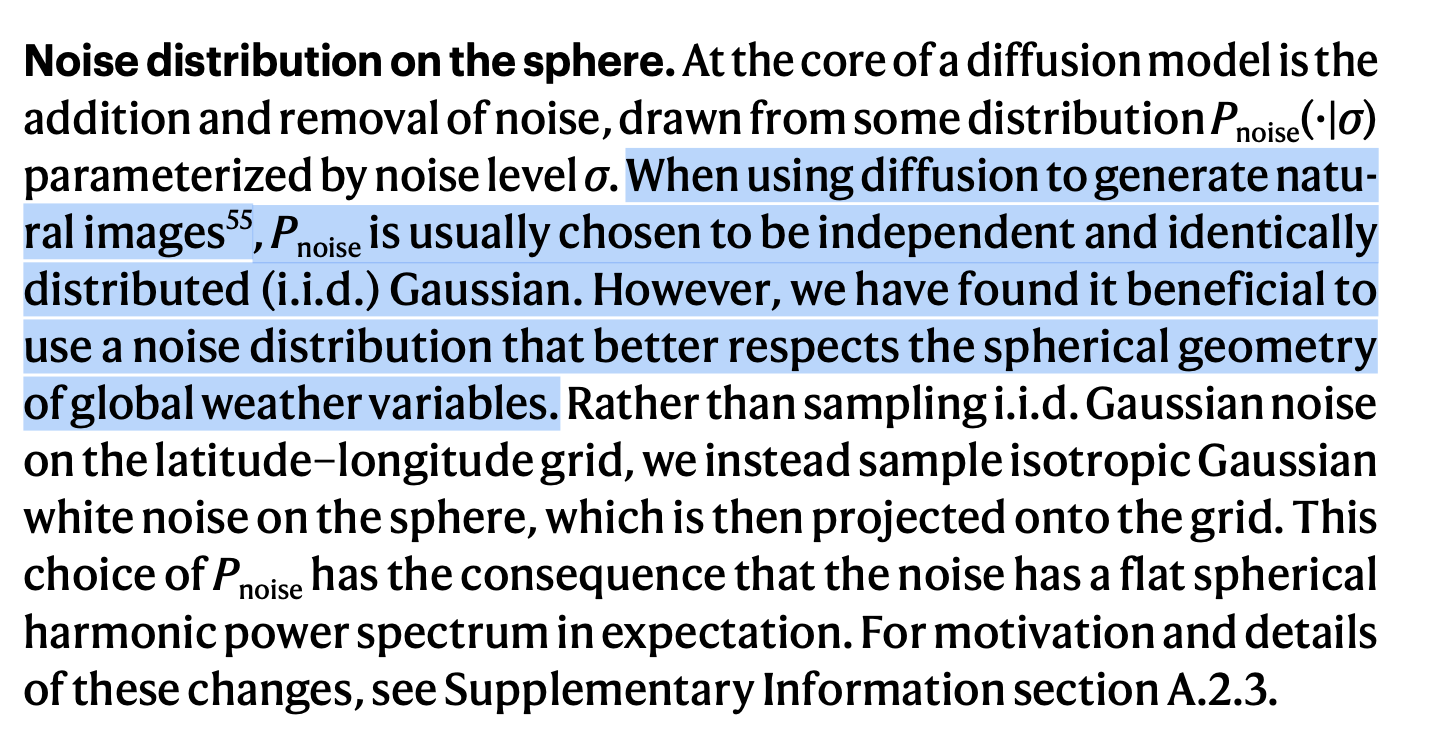
\includegraphics[width=.8\textwidth]{images/spherical_noise_distribution} 
\end{figure}
\end{frame}


\begin{frame}{Point \#3: Assessing Performance via Relative Economic Value (REV) curves}

Based on a \qq{cost-loss} decision model  for forecasts of binary events.
\vfill \pause 

A user must decide whether or not to prepare for an adverse weather event. Facing the event unprepared incurs an expense L (the `loss`). However, this loss can be avoided by preparing for the event with an expense C (the `cost`):

\begin{table}[h]
\centering
\begin{tabular}{c|cc}
 & Event doesn't happen & Event happens \\
\hline
No preparation made & 0 & L \\
Preparation made & C & C \\
\end{tabular}
\caption{Expenses under the cost-loss decision model.}
\label{tab:cost_loss}
\end{table}

\vfill
\pause 

The expected expense is:
\[E_{\text{forecast}} = (TP+FP) \cdot C + FN \cdot L \]

\end{frame}



\begin{frame}{Point \#3: Assessing Performance via Relative Economic Value (REV) curves}

We compare $E_{\text{forecast}}$, the expenses using the model forecast to 
\begin{itemize}
	\item $E_{\text{clim}}$, the expenses using climatology (long-term averages for this time of year) alone, and 
	\item $E_{\text{perfect}}$, the expenses incurred from a perfect forecast.
\end{itemize}

\pause
\vfill 

Using this we define the relative economic value as

\[ 
\boxed{
REV(C/L, q) = \frac{E_{\text{clim}} - E_{\text{forecast}}}{E_{\text{clim}} - E_{\text{perfect}}} 
}
\]
where $q$ is the probability threshold for preparing for an adverse weather event.  (The optimal choice is $q=C/L$.)

\pause 
\vfill 

\colorbox{blue!30}{\textbf{Remark.}} REV is 0 for a forecast based on climatology alone and 1 for a perfect forecast, so larger is better.

\end{frame}

\begin{frame}{Point \#3: Assessing Performance via Relative Economic Value (REV) curves}

We compare REV of Gencast with ENS, a state-of-the-art traditional weather forecasting method based on numerical weather prediction algorithms that approximately solve the equations that model atmospheric dynamics:

\begin{figure} 
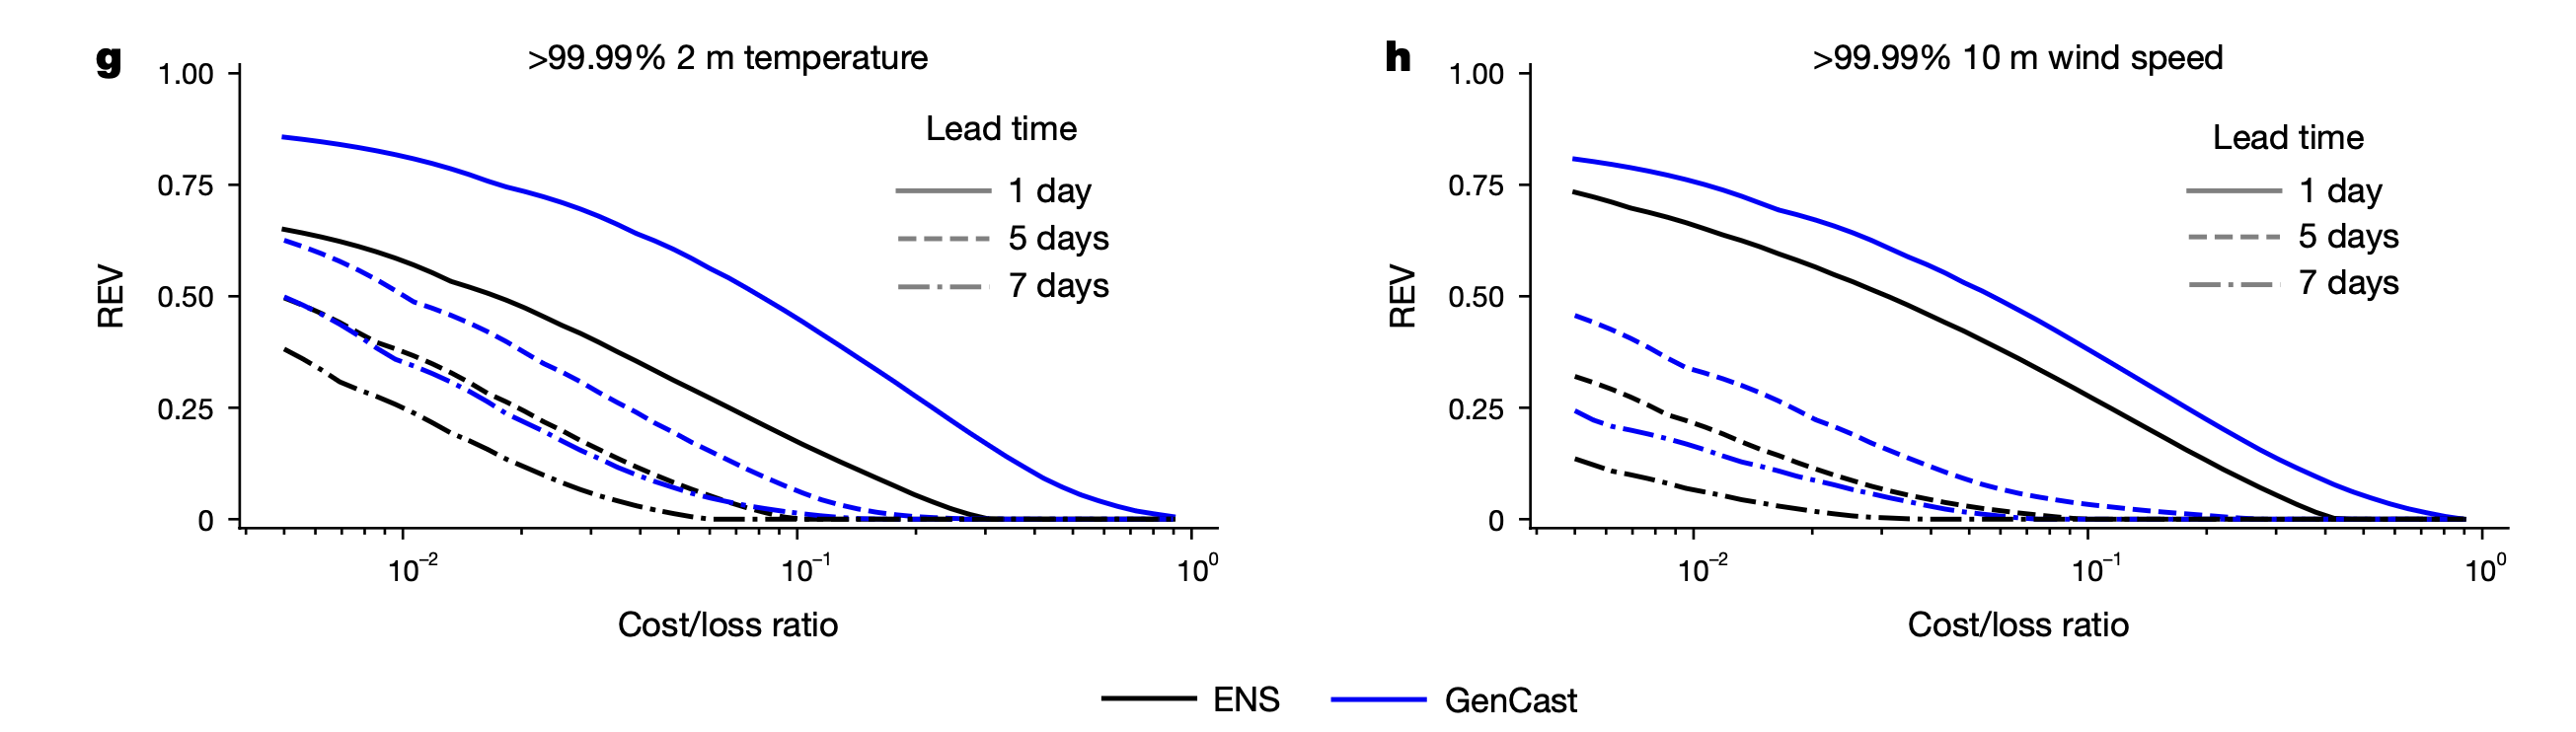
\includegraphics[width=\textwidth]{images/rev}
\caption{REV for predictions of the exceedance of the 99.99th percentile for 2m temperature and 10m wind speed, at lead times of 1 day, 5 days, and 7 days.} 
\end{figure}	
\end{frame}


\section{Class Discussion}


\begin{frame}{Format for Discussion}

\begin{enumerate}
	\item \textbf{Small group discussion:} Find 1-2 partners and discuss the paper.  For example, what did you
	%
	\begin{itemize}
		\item Like (or find interesting)?
		\item Dislike?
		\item Find confusing?
		\item Feel you'd do differently?
	\end{itemize}
	%
	\item \textbf{Classroom discussion:} We'll circle around and report on our evaluations, and then launch into a class discussion.
\end{enumerate}
	
\end{frame}



\end{document}

